\section{Incrementally maintain classifiers}
%road map
In this section, some recent works on incrementally maintaining materialized classifier parameters in database are presented, which initially originates from \cite{deshpande2006mauvedb} and follows by \cite{koc2011incrementally}. Both \cite{deshpande2006mauvedb} and \cite{koc2011incrementally} develop a system (MauveDB vs Hazy) to store typical statistical model parameters as database view in RDBMS and update the views incrementally when raw data are modified.   

\subsection{MauveDB}
%brief description to MauveDB
MauveDB primarily deals with wireless sensor network applications, where data are collected through underlying sensors, fitted with typical statistic model such as regression-based model and interpolation-based model and used for estimating missing or future results. The statistic models learned with those raw data are materialized as {\em model-based views}, which are created with a high-level SQL-like language. Due to the addition or removal of the sensors, raw data are updated constantly, which requires efficient view maintenance strategies. The details of how {\em model-based views} are defined, updated and queried for prediction are provided as follows, which highly depend on the types of statistical model.

\subsubsection{Basic notations}
We will use capitalized letters (e.g. $H$) to denote matrix, capitalized bold letters (e.g. $\textbf{T}$) to denote tables, lowercase letters (e.g. $x$ and $y$) to denote scalar value, bold lowercase letters (e.g. $\textbf{x}$) to denote variables, lowercase letters with bar (e.g. $\bar{w}$) to denote a vector, $f(*)$ to denote functions ($*$ represents arguments of function $f$). Besides, we use $H_{i,j}$ to denote the value at cell $(i,j)$ in matrix $H$ and use $\bar{w}_i$ to denote $i_{th}$ element in vector $\bar{w}$. Based on those notations, we provide notations for each model as follows.

\paragraph{Regression model}
A regression model is usually written as the following form:
\begin{equation}
t=\sum_{i=1}^kw_ih_i(*)
\end{equation}
where $h_i$ represents {\em basis function}, which is a monomial of {\em predictor variables} while $w_i$ represents coefficient of those monomials and $t$ is the {\em response variable}.

For example, in wireless sensor network application, temperature is measured at a 2D-space with coordinate $x$ and $y$, which can be computed with the following typical polynomial of the two predicator variables:

\begin{equation}
temp=w_1 + w_2x+w_3x^2 + w_4y+w_5y^2
\end{equation}
where the basis functions are $\{h_1(x,y), h_2(x,y), h_3(x,y),h_4(x,y), h_5(x,y)\}=\{1, x, x^2, y, y^2\}$

Given a set of data observed from the underlying wireless sensors located at different positions, $\{x_j,y_j,temp_j\}(j=1,2,\dots,n)$, the coefficients $\bar{w}^* = \{w_1,w_2,\dots,w_k\}$ are estimated with the following linear system:
\begin{equation}\label{eq: regression_solve}
    H^TH\bar{w}^*=H^T\bar{f}
\end{equation}

where $H$ is:
\begin{equation}
    H=\begin{bmatrix}
h_1(x_1,y_1) & h_2(x_1,y_1) &\dots &h_k(x_1,y_1)\\
h_1(x_2,y_2) & h_2(x_2,y_2) &\dots &h_k(x_2,y_2)\\
\dots\\
h_1(x_n,y_n) & h_2(x_n,y_n) &\dots &h_k(x_n,y_n)
\end{bmatrix}
\end{equation}

and $\bar{f}$ is:

\begin{equation}
    \bar{f} = \{temp_1, temp_2,\dots, temp_n\}^T
\end{equation}

In general, $H$ will be a matrix which represents data sets of $n$ data points with $k$ features while $\bar{f}$ represents the label vectors.

\paragraph{Interpolation model} 

The goal of interpolation is to estimate missing values of response variables given a value of predictor variable, which does not exist in the set of existing value pair for predictor variable and response variable. Specifically, given a variable pair $(\textbf{t},\textbf{v})$ and a set of value pairs for those two variables, $(t_i, v_i)(i=1,2,\dots,n)$ observed from sensors are then used to estimate value $v'$ of variable $V$ given a value $t'$ of variable $T$ $(t_j< t' < t_{j+1})$. Usually, {\em linear interpolation} is used. So $v'$ is estimated with value pair $(t_j, v_j)$ and $(t_{j+1}, v_{j+1})$ as follows:
\begin{equation}\label{eq: interpolation}
    v'= v_j + (v_{j+1}-v_j)\times\frac{t'-t_j}{t_{j+1}-t_j}
\end{equation}




\subsubsection{View definition}

MauveDB developed an declarative SQL-like language for users to define model-based view, which is exemplified in Figure \ref{fig:MauveDB_view_def}. Although different models cannot be manipulated in exactly the same way due to their different characteristics, the commonalities are still leveraged in this language. 

In Figure \ref{fig:MauveDB_view_def}, examples of regression-based view and Interpolation-based view definitions are presented in (i) and (ii) respectively. Same as way to create other database views, the view schemas, where the raw data comes from to construct the views (represented by \textit{SELECT}, \textit{FROM}) and what conditions the raw data should satisfy (represented by \textit{WHERE}) should be declared in the view definition statements. The model types (\textit{FIT} and \textit{INTERPOLATE} for regression and interpolation respectively) should be also specified along with partitions of raw data on each of which the models are trained (\textit{FOR EACH}) and other model-related information (such as base function for regression model, represented by \textit{BASE}). After executing statements shown in Figure \ref{fig:MauveDB_view_def}, {\em model-based views} are then created and stored in the RDBMS as relational tables.


\begin{figure}
    \centering
    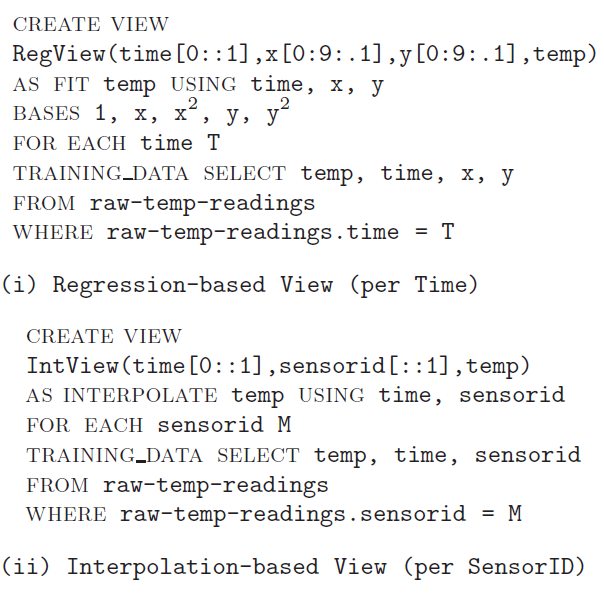
\includegraphics[width=8cm, height=8cm]{Figures/MauveDB_create_view.png}
    \caption{Define views in MauveDB}
    \label{fig:MauveDB_view_def}
\end{figure}

\subsubsection{View maintenance}
%High-level descriptions of view maintenance strategies
When the new data are available, the updates should be reflected on the model-based views. Four different strategies are developed for this purpose and their trade-offs are discussed with extensive experiments. The details of the four view maintenance strategies are introduced in this section.

\textit{Strategy 1: Materialize the views}
A naive way is simply to construct the models and materialize the model parameters as views in the database, which can avoid unnecessary query execution time when users want to retrieve the ``exact'' model information. However, such views may incur high space overhead and pose a challenge in refreshing the model as new data comes.

\textit{Strategy 2: Always use the base data}
This strategy goes to another extreme without materialization at all in the database, which can obviously make query processing very expensive since recomputating the view content is necessary every time when queries are evaluated. 

\textit{Strategy 3: Partial materialization}
Somewhere in-between is to partially materialize the view content, which simply caches parts of the views that have been computed by certain queries. When the views are about to be refreshed, the corresponding cached contents in memory will be invalidated.

\textit{Strategy 4: Materialize an intermediate representation}
Some intermediate representations are materialized in this strategy by leveraging some nice properties of regression model and interpolation model, which have been an efficient solution experimentally and are presented as follows for the two models respectively.

For regression model, recall that the optimal coefficients can be solved with Equation \ref{eq: regression_solve}. The intermediate representation for it can be simply the materialization of matrix $H^TH$ and $H^T\bar{f}$, which can be beneficial in various aspects. First, the dimensions of the two matrices only rely on the total number of features, which thus won't lead to large space overhead. Besides, efficient updates to the two matrices are achievable since they are computed with linear operators, i.e. matrix multiplications and additions. A newly generated data point $(x',y', temp')$ can trigger the update of $H^TH$ and $H^T\bar{f}$ as follows:
\begin{equation}
    (H^TH)^{new}_{i,j} = (H^TH)^{old}_{i,j} + h_i(x',y')*h_j(x',y')
\end{equation}
\begin{equation}
    (H^T\bar{f})^{new}_i = (H^T\bar{f})^{old}_i + h_i(x',y')*temp'
\end{equation}

Once the user queries arrive, the coefficient $\bar{w}$ is computed with the following expression:
\begin{equation}
    \bar{w}^*=(H^TH)^{-1}H^T\bar{f}
\end{equation}

which can be computed with time complexity $Q(k^3)$ where $k$ is the total number of features.

For interpolation model, following the example shown in Figure \ref{fig:MauveDB_view_def}, the data in the interpolation-based view $\textbf{V}$ will be of the form $(\textbf{t}, \textbf{v})$ where $\textbf{t}$ represents time while $\textbf{v}$ represents observed value by the sensors. Unlike regression mode, its intermediate representations are not additional data but some additional data structure for searching the values of variable $\textbf{t}$. In order to efficiently estimate the sensor values for time $t'$ which is missing from the view instance but queried by users, the closest values $t_{-}$ and $t_{+}$ (along with the corresponding sensor values $v_{-}$ and $v_{+}$) to $t'$ are retrieved with the auxillary data structure such that $t'$ lies in the interval $(t_{-}, t_{+})$ with no other $\textbf{t}$ value from $\textbf{V}$ in it. So the estimated sensor value at time $t'$ can be computed using Equation \ref{eq: interpolation}.

The specific choice of strategies in practice depends on various factors, such as the query workload, data statistics and types of models. The trade-off between the four strategies are experimentally explored with extensive experiments in \cite{deshpande2006mauvedb}, which shows that the strategy 4 performs best in most scenarios while strategy 1 can actually outperform others in some cases.

\subsection{Hazy}



\section{Incrementally compute matrix programs}


\section{Incrementally derive new models with existing models}